Um die Funktionsweise beider Algorithmen zu belegen wurden beide Methoden einerseits auf ihre Robsutheit und andrerseites auf ihre Performance getestet. Im folgenden Kapitel wird zunächst das zum Testen verwendete Setup beschrieben. Anschliessend erfolgt die Auswertung der erlangten Testergebnisse. Zuletzt werden weitere Tests durchgeführt welche das System kritischen Situationen testen soll.

% ---------------------- section -----------------------
\section{Testsetup}
\label{sec:test_setup}

Bei der Durchführung der Tests befinden sich die Kameras statisch im Raum. Die zu erkennenden Hindernisse werden innerhalb und ausserhalb der zu erkennenden Reichweite platziert, wobei die Ausrichtung der Hindernisse teils zufällig, teils bewusst an kritischen Positionen erfolgt, um ein reales Anwendungsszenarien passend zu simulieren. Ein aufgenommenes Testset besteht dabei aus beiden Bildern der Kamera, der normalisierten Disparity Map sowie eine komplette Pointcloud dieser um etwaige Fehler der Algorithmen leichter erkennen zu können, sowie den geloggten Pointclouds der Hinderniserkennung. Weiterhin werden diverse Parameter gespeichert, wie die Anzahl der erkannten Hinderniselemente, sowie deren Disparitäten.\\

\noindent
Der zu erkennende Bereich wurde auf $0,2$ bis $1,5$ Meter definiert. Dies entspricht einem Szenario in welchem das System auch aufgrund der hohen Framerate der Erkennung angewendet werden kann. Eine Erweiterung dessen auf beispielsweise $2.0$ Meter wurde nicht durchgeführt, da der Algorithmus auch bei großen Entfernungen robuste Werte in der Distanzberechnung liefert \cite{hilleralhallak}.
Das dabei erreichte Sichtfeld nach der Anwendug der ROI auf die Disparity Map (siehe \ref{sec:preprocessing}) beträgt $50^{\circ}$ auf horizontaler Achse und $38^{\circ}$ vertikal. Dies ist in Abbildung (REF) visualisiert.
	% TODO sichtfeld durch disparity map & vergleich zum ursprünglichen sichtfeld

\noindent
Ein aufgenommenes Testset besteht aus jeweils 12 Testbildern. Für jede Methode wurden drei verschiedene Hindernisgrößen getestet, groß, klein und winzige Hindernisse. Anhand dieser wird ausgewertet welche minimale, maximale sowie mittlere Disparität, und daraus resultierende Distanz erkannt wird.\\

\noindent
Weitere Tests beinhalten die Erkennung winziger Hindernisse unter Veränderung der \emph{SGBM} Parameter. Dabei wird unter anderem untersucht ob beispielsweise eine verringerte Blockgröße Einfluss auf die Erkennung kleiner Bereiche nimmt. Des Weiteren wird die Zeit für die Hinderniserkennung eines Frames untersucht um eine durchschnittliche Zeit für die Erkennung sowie die daraus resultierende Framerate zu ermitteln. Dies geschieht einerseits durch die Erkennung eines Hindernisses, welches sich über das gesamte Bild ausbreitet, andererseits für nur ein Teilelement jeder Erkennungsmethode (Subimage, Samplepoint).\\
Zudem wird geprüft inwiefern die Algorithmen mit Limitierungen des \emph{SGBM} umgehen können. Dazu zählen die Erkennung bei spiegelnden, reflektierenden und durchsichtigen Flächen, sowie die Erkennung schwach texturierter Hindernisse.\\

% kameras statisch im raum
% hindernisse innerhalb der zu erkennenden reichweite platziert
% ausrichtung der hinernisse zum teil zufällig
% teils bewusst an kritischen positionen platizert
% für jeden Frame werden Informationen geloggt wie anzahl der erkannten hindernisse sowie position der hindernisse im raum
% für jeden frame wird eine vollständige pointcloud berechnet um etwaige fehler zu erkennen
% verschiedene hindernisgrößen gross klein winzig
% jeweils 12 testbilder
% range auf 0.2 - 1.5 meter festgelegt --> real life szenario

% weitere tests:
	% erkennung von kleinen hindernissen mithilfe veränderter sgbm parameter
	% zeit die fuer die ausführung der detectObstacles funktion benötigt wird
	% können auch extreme situationen wie durchsichtige flächen erkannt werden?
		% spiegelnd
	% erkennung von wenig texturierten hindernissen
	% 

% ---------------------- section -----------------------
\section{Evaluierung Subimage Detection}
\label{sec:evaluierung_subimage}

    \subsection{Robustheit}
    \label{subsec:subimage_robustheit}
    Hinsichtlich der Robustheit wurden beide Algorithmen nach demselben Schema untersucht. Der in Abschnitt \ref{sec:test_setup} beschriebene Testablauf beschreibt 3 verschiedene Hindernisgrößen. Tabelle \ref{tbl:obstacle_sizes} zeigt sowohl die Maße der Hindernisse als auch die Fläche in $cm/cm^2$ auf.
    
	\begin{table}[h]
	\centering
	\begin{tabular}{|l|c|c|c|c|}
	\hline
	Hindernis   & Radius & Länge & Breite & Fläche \\
	\hline
	Groß   		&   -    & 53.5  & 43.0   & 2300.5 \\
	\hline
	Mittel 		& 	-    & 16.0  & 14.5   & 232.0\\
	\hline
	Winzig		& 2.5	 &   -   &   -    & 19.6 \\
	\hline	
	\end{tabular}
	\label{tbl:obstacle_sizes}
	\caption{Maße der verschiedenen genutzten Hindernisse}
	\end{table}
	
	\noindent
	Während der Tests wurde für jedes aufgenommene Einzelbild die reale Distanz gemessen. Der dabei verwendete Referenzpunkt befand sich in der Mitte des zu erkenneden Hindernisses, da diese nicht zwangsläufig orthogonal zur Bildebene platziert wurden. Somit entspricht die gemessene Distanz der mittleren Distanz welche sich aus allen gefundenen Bereichen eines Bildes zusammensetzt. Während der Aufnahme sind die jeweiligen Einzelbilder der linken und rechten Kamera sowie die berechnete Disparity Map sichtbar. Weiterhin ist ein weiterer Anzeigemodus verfügbar welcher die gefundenen Hindernisse innerhalb der Tiefenkarte markiert (siehe Abbildung \ref{fig:test_viewing}). Weiterhin kann jede erstellte Hindernis-Pointcloud im Nachhinein gerendert werden um einen überblick über die Ergebnisse des Algorithmus zu erhalten.\\
	
	\noindent
	\textbf{Großes Hindernis:}\\
	\begin{figure}[h]
		\centering
		\begin{tabular}{c c}
		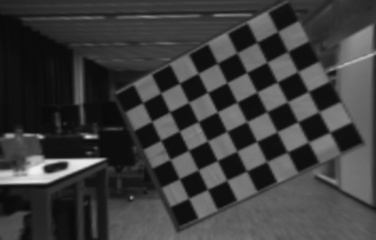
\includegraphics[width=5.0cm]{img/evaluation/test_set/_test_3_left}&
		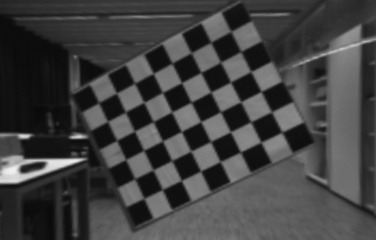
\includegraphics[width=5.0cm]{img/evaluation/test_set/_test_3_right}\\
		(a) linkes Kamerabild & (b) rechtes Kamerabild\\
		
\includegraphics[width=5.0cm]{img/evaluation/test_set/_test_3_disparity}&
	    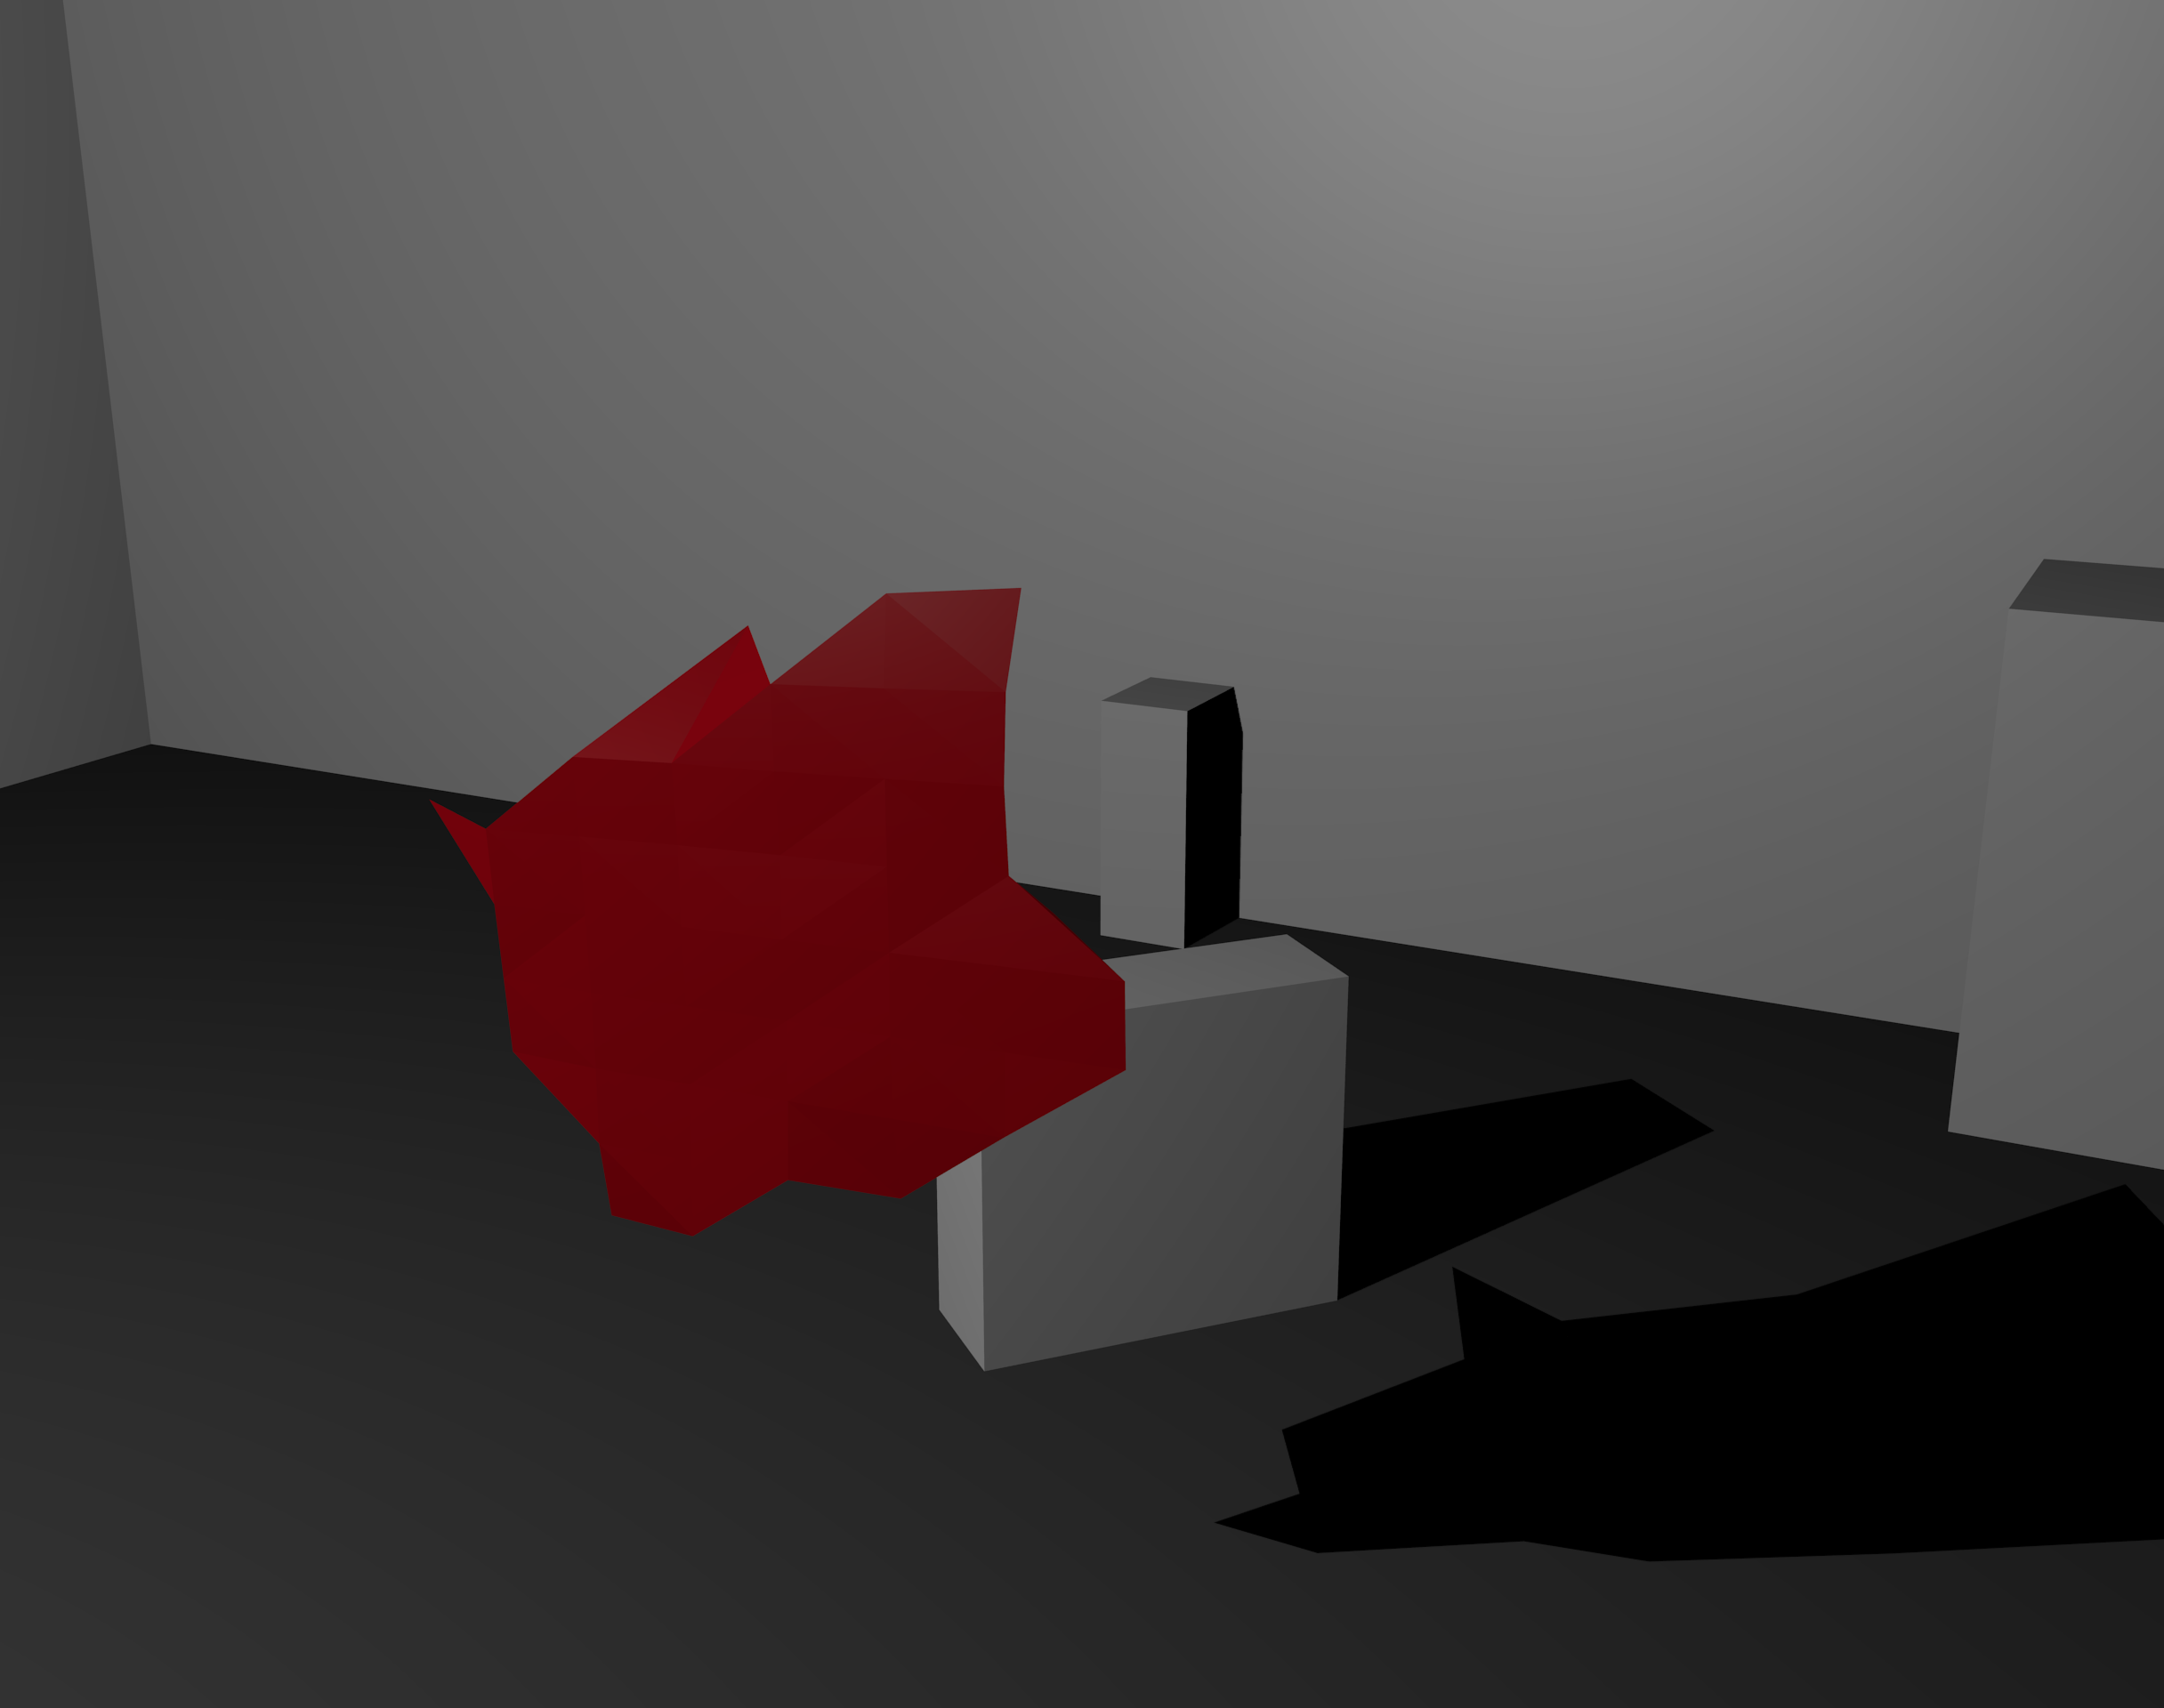
\includegraphics[width=5.0cm]{img/evaluation/test_set/rendered_obstacle}\\
		(c) Anzeigemodus Hindernis & (d) Hindernis Pointcloud als Mesh
		\end{tabular}
		\caption{Abbildungen (a) - (c) zeigen die sichtbaren Bilder während der Testaufnahme. (c) zeigt eine als Mesh gerenderte Pointcloud}
		\label{fig:test_viewing}
	\end{figure}
   	% TODO hindernisform: was ist daran gut / schlecht vielleicht
    
    \noindent
	Im ersten Test wurde das große Hindernis gewählt, dabei wurde mithilfe der dargestellten Hindernisse auf der Disparity Map überprüft ob sich die erkannten Hindernisse innerhalb des Gefahrenbereichs befinden. Um auch kritische Bereiche zu testen wurde das Hindernis zudem zu Teilen außerhalb dieser platziert. Aus den 12 aufgenommenen Bildern des Testsets ergaben sich die in Abbildung \ref{fig:eval_big} (a) sichtbaren Ergebnisse.\\
    
	% den gespeicherten weltdistanzen
	% den daraus resultierentden median werten der distanz
		% berechnet und gemessen
	% werden Hindernisse erkannt
	% wie hoch ist der drift zwischen den einzelnen sets
	% vielleicht standartabweichung betrachten
	% für jedes set einzeln
	% woher kommen die drifts 
		% (person im bild bei der bildaufnahme
		% hindernisse im winkel gehalten --> geneigt
	% trotzallem wurde jedes hindernis erkannt
	% abweichung entsteht einerseits durch besagten drift durch beschriebene gruende
		    
	\begin{figure}[h]
		\centering
		\begin{tabular}{cc}
		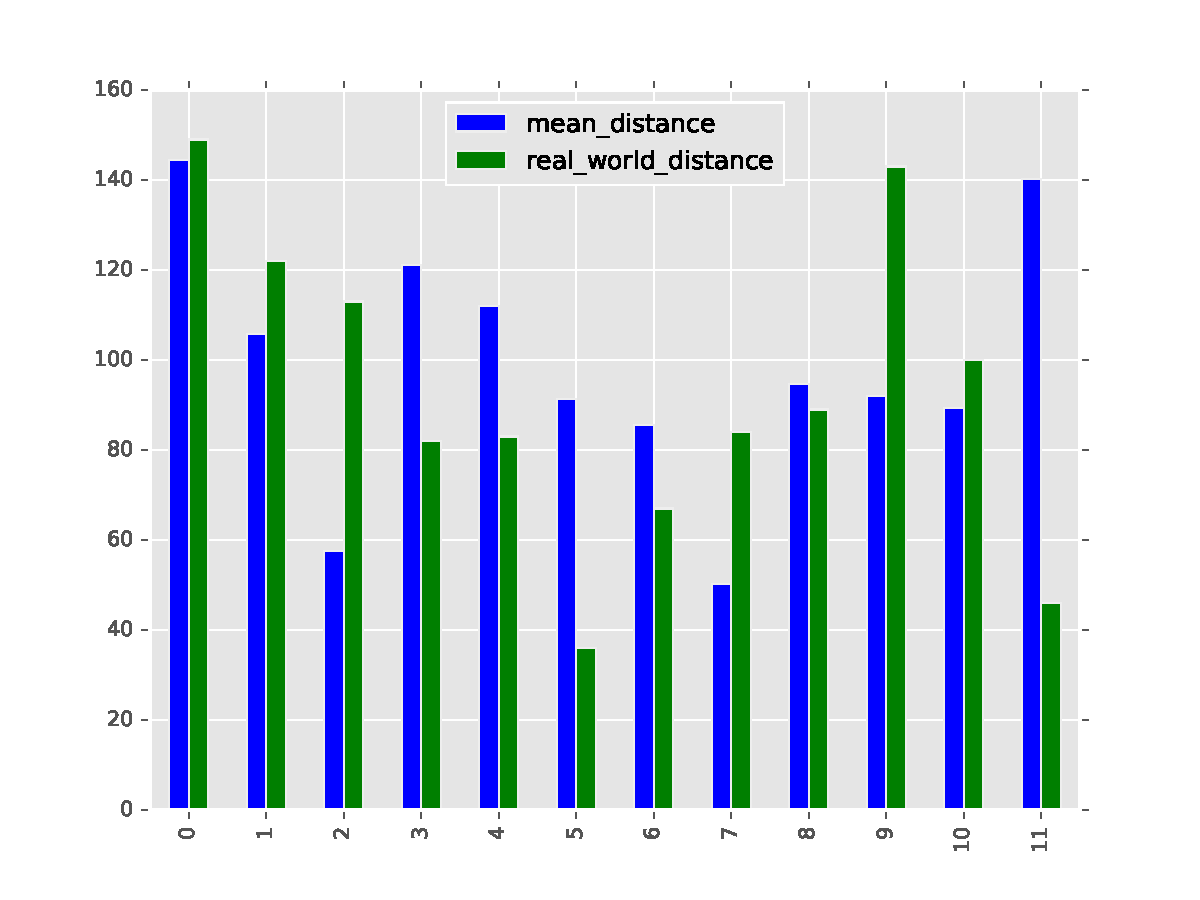
\includegraphics[width=7cm]{img/evaluation/big_bar}&
		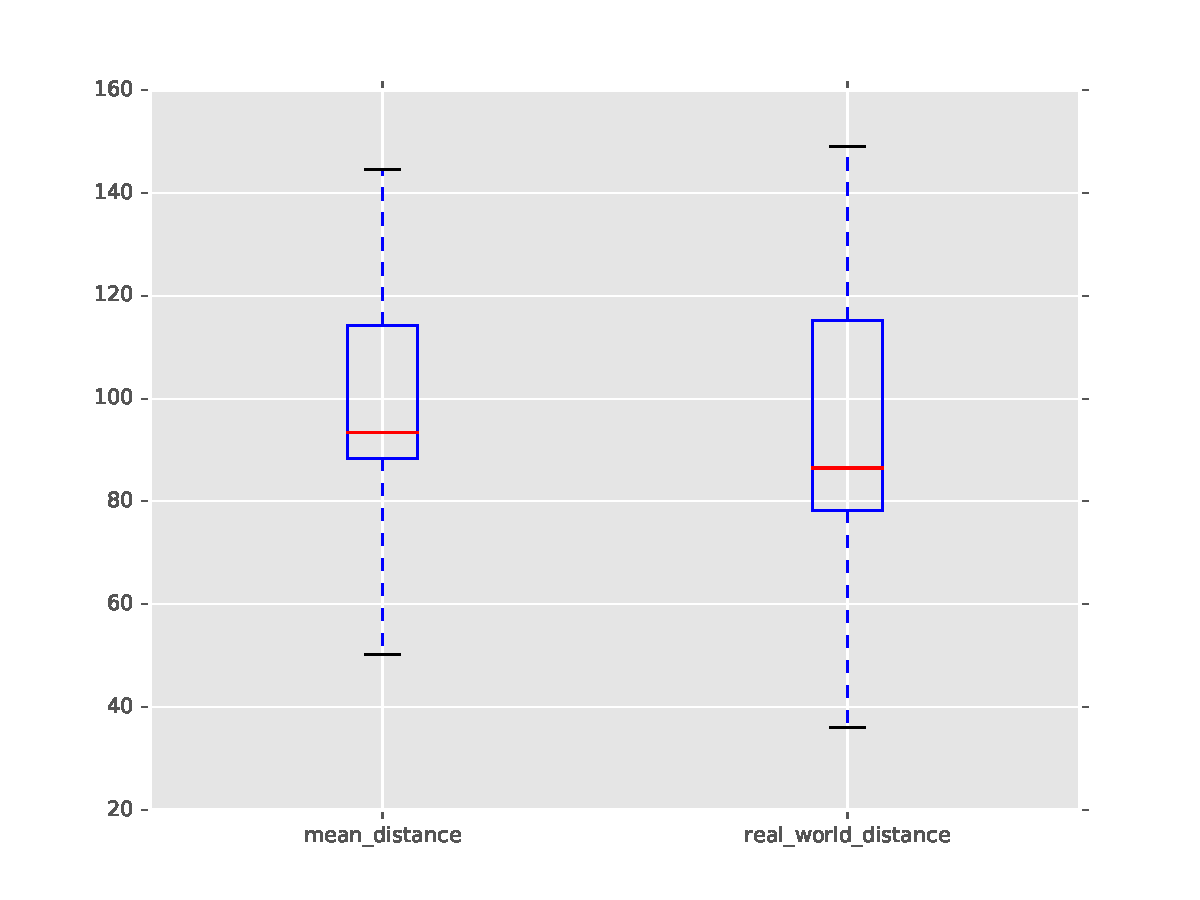
\includegraphics[width=7cm]{img/evaluation/big_box}\\
		 (a) & (b)
		\end{tabular}
		\caption{}
	    \label{fig:eval_big}
	\end{figure}
	
	\noindent
	Wie aus dieser zu erkennen wurde in nahezu allen Frames das Hindernis richtig erkannt. Die berechneten Distanzen stimmen, ausgenommen Bild 5, 6 und 11, mit den real gemessenen überein. Minimale Abweichungen können in diesem Fall als Messungenauigkeit ignoriert werden, da der Mittelpunkt zwischen der minimalen und maximalen Objektdistanz kein statisch gleichbleibender Punkt ist. In Bild 5 kann eine erkannt werden das eine zu geringe Distanz einerseits zu Bildfehlern aufgrund unklarer Korrespondenz führen kann, und andererseits die gemittelte Distanz nicht mehr mit der realen übereinstimmt. Abbildung \ref{fig:eval_big_fails} zeigt eben diese Probleme auf. In Bild 6 befindet sich eine weitere Person innerhalb der Gefahrenzone. Diese wird ebenfalls erkannt, was dazu führt, dass sich der Median der Distanzen aus denen der im Hintergrund befindlichen Person und dem Objekt im Vordergrund zusammensetzt.
	
	\begin{figure}[h]
		\centering
		\begin{tabular}{cc}
		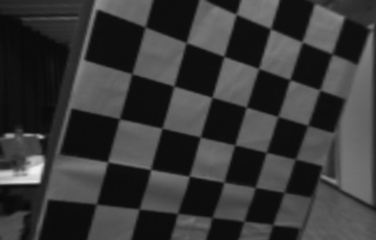
\includegraphics[width=5cm]{img/evaluation/big_5_left}&
		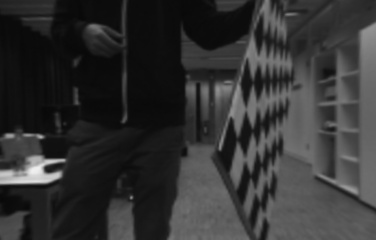
\includegraphics[width=5cm]{img/evaluation/big_6_left}\\
		(a) Frame 6 &  (b) Frame 5
		\end{tabular}
		\caption{}
	    \label{fig:eval_big_fails}
	\end{figure}

	\noindent
	Auch im in Abbildung \ref{fig:eval_big} (b) abgebildeten Boxplot lässt sich erkennen, dass der Median beider gemessenen Distanzen, mit geringen Abweichungen, nahezu gleich ist. Auch die minimal und maximal Werte befinden sich, ebenfalls mit vernachlässigbarer Abweichungen auf derselben Gerade. Lediglich das untere Quartil der real gemessenen Distanz weicht um $10 cm$ von der der gemessenen ab. Dies resultiert aus Frames in welchen die berechnete Distanz höher ist als die gemessene.\\

	\noindent
	\textbf{Mittleres Hindernis:}\\
	\begin{figure}[h]
		\centering
		\begin{tabular}{cc}
		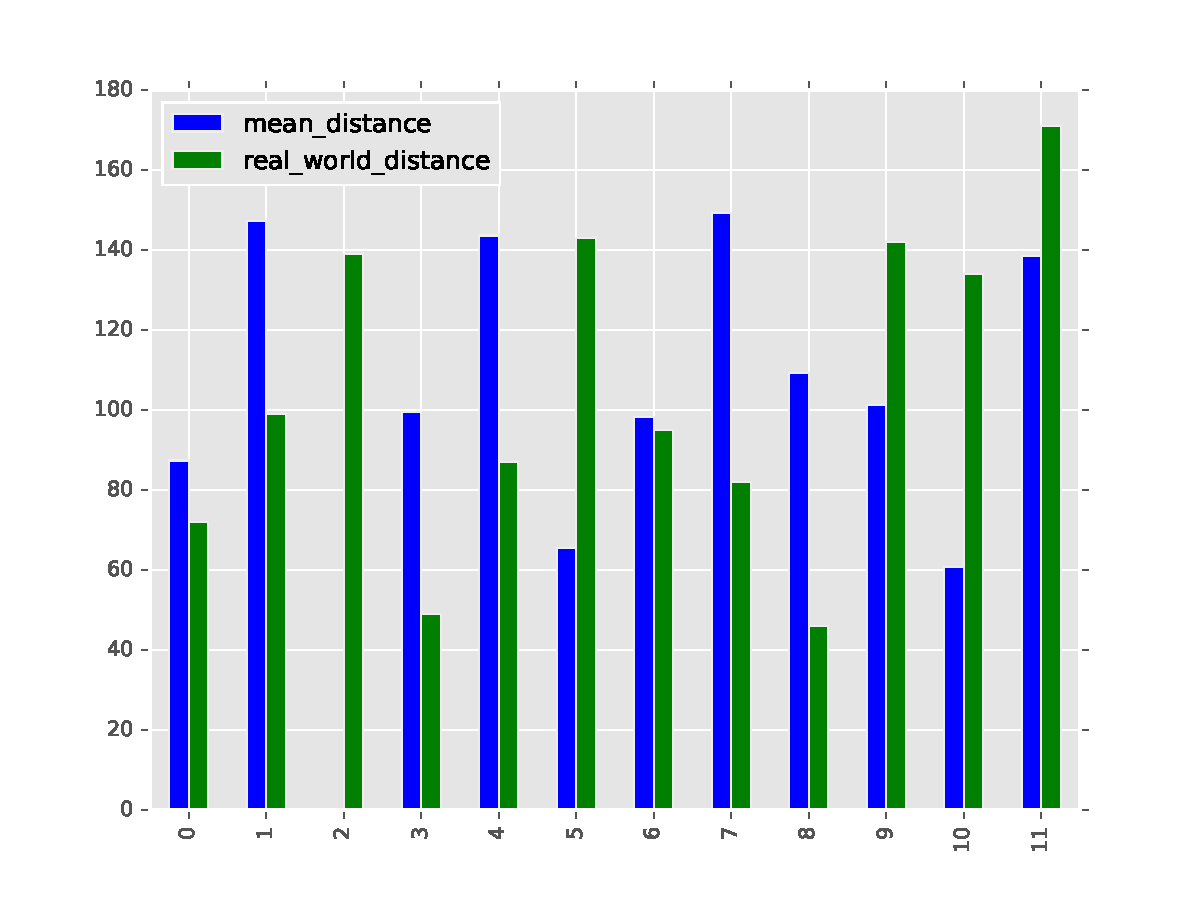
\includegraphics[width=7cm]{img/evaluation/medium_bar}&
		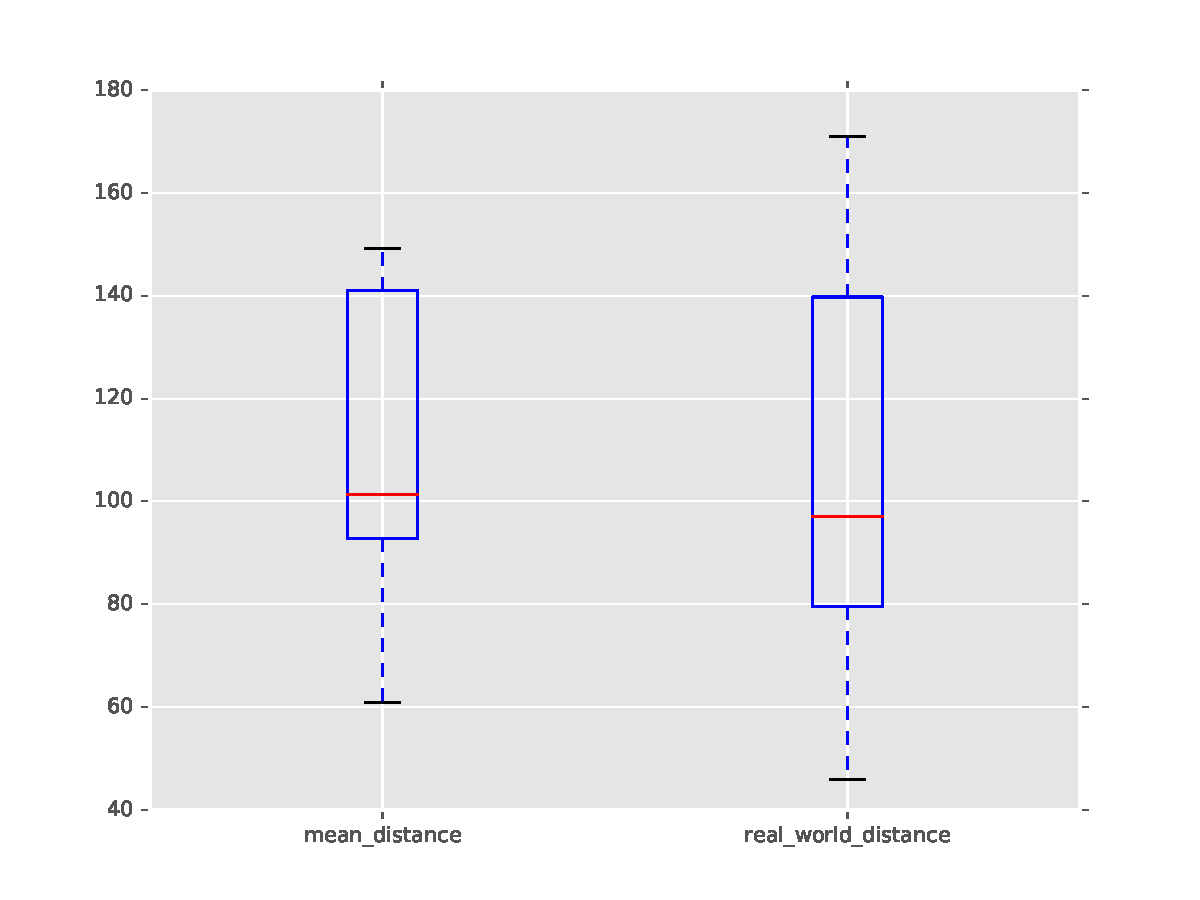
\includegraphics[width=7cm]{img/evaluation/medium_box}\\
		(a) &  (b)
		\end{tabular}
	    \caption{}
	    \label{fig:eval_medium}
	\end{figure}
	
	\noindent
	Auch die Erkennung mittlerer Hindernisse durch den Algorithmus war in nahezu allen Fällen erfolgreich. Ein auffälliges Detail im Vergleich zu den Ergebnissen des großen Hindernisses ist die höhere Differenz aus berechneter und gemessener Distanz. Lediglich Frame 1, 2, 5 und 9 zeigen eine geringere Abweichung. Das getestete Objekt befand sich während der Tests an einem durchsichtigen Plexiglas Stab. Dieser ist teilweise auch als Hindernis erkannt worden. Im Fall von Frame 0 umfasst das Objekt insgesamt 4 Subimages in denen es erkannt wurde. Ein fünftes Subimage wurde als Resultat des Stabes ebenfalls erkannt. Dies ist nicht der alleinige Auslöser der hohen Abweichungen, jedoch ein geringer Teil, da der Median der gesamten Teilmatrix gerade so hoch ist um vom Algorithmus als Hindernis erkannt zu werden. Die Orientierung des Hindernisses in Bild 3 ist sowohl in $x$ als auch in $z$ Achse rotiert. Dies resultiert in einer Erkennung der einzelnen Flächen, welche geometrisch weiter entfernt sind, und dem Messpunkt welcher auf der vorderen Ebene des Objektes platziert war (siehe Abbildung \ref{fig:eval_medium_fails} (b)). 
	
		\begin{figure}[h]
			\centering
			\begin{tabular}{cc}
			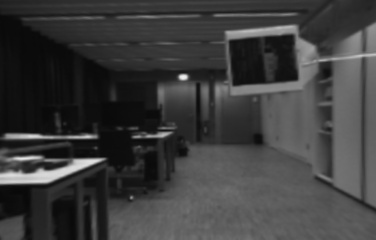
\includegraphics[width=5cm]{img/evaluation/medium_0_left}&
			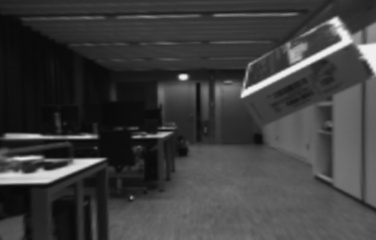
\includegraphics[width=5cm]{img/evaluation/medium_3_left}\\
			(a) Frame 0 &  (b) Frame 3
			\end{tabular}
			\caption{}
		    \label{fig:eval_medium_fails}
		\end{figure}
	
	\noindent
	Selbiges Resultat lässt sich in den Frames 4, 6 und 7 erkennen. In Frame 8 war das eigentlich Objekt nur teilweise im Bild zu erkennen, das eigentlich erkannte Hindernis ist in diesem Fall der beschriebene Befestigungsstab. Frame 8 enthält keine Informationen zu einem erkannten Hindernis, da sich das Hindernis direkt an der Grenze des Gefahrenbereichs befand.	Eben diese Ergebnisse sind auch in Abbildung \ref{fig:eval_medium} (sb) sichtbar, das Maximum der realen Distanz resultiert dabei aus dem nicht erkannten Hindernis in Frame 11.\\
	
	\noindent
	\textbf{Winziges Hindernis:}\\
	\begin{figure}[h]
		\centering
		\begin{tabular}{cc}
		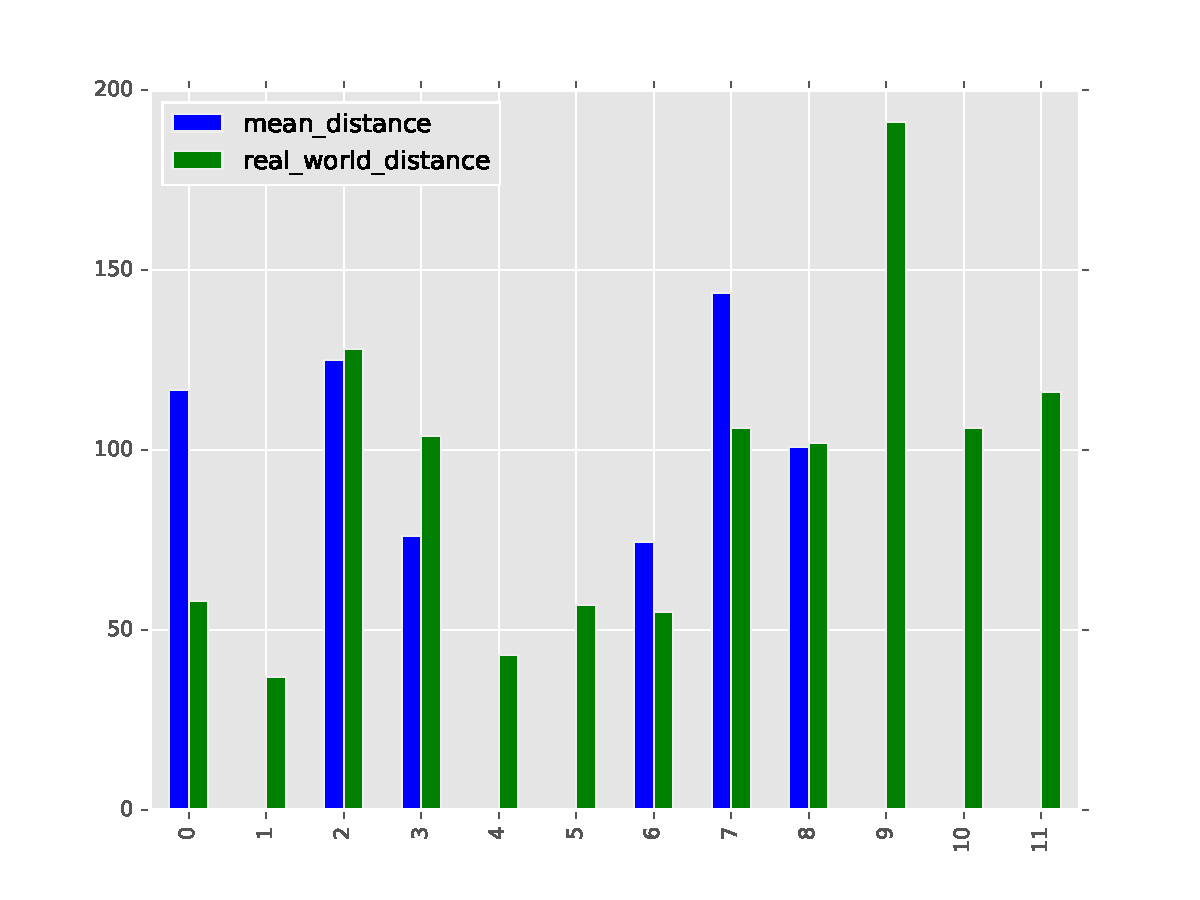
\includegraphics[width=7cm]{img/evaluation/tiny_bar}&
		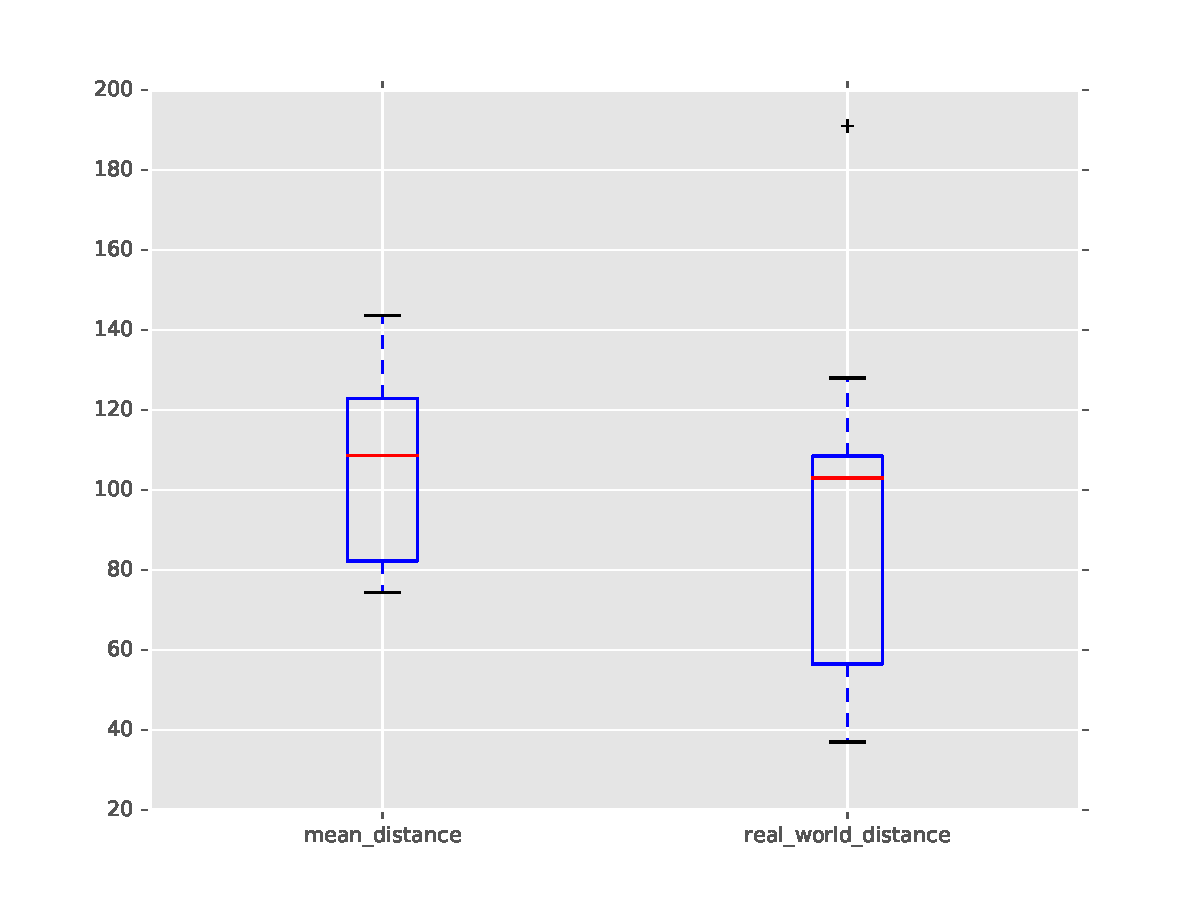
\includegraphics[width=7cm]{img/evaluation/tiny_box}\\
		(a)	& (b)
		\end{tabular}
	    \caption{}
	    \label{fig:eval_tiny}
	\end{figure}
	
	Die Erkennung Winziger Hindernisse gestaltet sich aufgrund diverser Faktoren schwer. Ein limitierender Faktor ist die Fläche, wenn ein einzeles Hindernis so klein ist, dass es während der Mittelwertberechnung aufgrund der umliegenden Disparitäten untergeht. Dies macht sich in nahezu allen getesteten Bildern bemerkbar. In den Frames 2 und 3 sowie 7-10 wurde das Hindernis nicht erkannt, da es sich an einer Kreuzung verschiedener Subimages befand, dadurch wird der Median aller Teilmatrizen nicht signifikant beeinflusst. In Frame 6 wurde das Objekt um um 90$^{\circ}$ rotiert, sodass nur noch eine Seitenansicht dessen vorhanden war. Dies reicht zwar in diesem Frame zur Erkennung des Hindernisses aus, jedoch wurde im selben Frame auch der Stab als Hindernis erkannt. Auch der in Abbildung \ref{fig:eval_tiny} (b) dargestellte Boxplot zeigt, das signifikant größere Distanzen erkannt wurden als sie in den realen Messungen vorkommen. Auch dieser Punkt lässt sich durch die Nutzung des Mittelwertes innerhalb der Subimages begründen.

% ---------------------- section -----------------------
\section{Evaluierung Samplepoint Detection}
\label{sec:evaluierung_samplepoint}

    \subsection{Robustheit}
    \label{subsec:samplepoint_robustheit}    
